\documentclass[12pt]{article}
\usepackage{fullpage,graphicx,psfrag,amsmath,amsfonts,verbatim}
\usepackage[small,bf]{caption}
\usepackage{float}

\input defs.tex

\title{\textbf{Assignment 16 CME 241}}
\author{Taylor Howell}

\begin{document}
\maketitle

\newpage

\section{Monte Carlo Policy Gradient (REINFORCE)}
For this problem I implemented REINFORCE in Julia. I initially applied the algorithm to the asset allocation problem from chapter 7 (\texttt{q1_asset_allocation.jl}). I parameterized my policy using a Gaussian in order optimize over the continuous action space. However, the algorithm kept diverging. I then implemented the short-corridor grid world Markov decision process from Sutton and Barto and was able to approximately solve the problem using REINFORCE (\texttt{short_corridor_reinforce.jl}).

\begin{figure}[H]
	\centering
	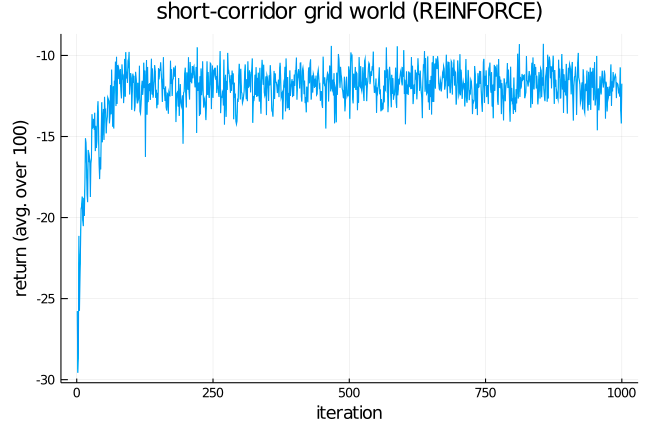
\includegraphics[width=.75\textwidth]{figures/sc_gw_reinforce.png}
	\caption{Return for short-corridor grid world during training with REINFORCE.}
	\label{}
\end{figure}

\section{Actor-Critic Eligibility Traces}

\end{document}
